\documentclass[a4paper, 12pt]{article}

\usepackage[T2A]{fontenc}
\usepackage[utf8]{inputenc}
\usepackage[english,russian]{babel}
\usepackage{amsmath, amsfonts, amssymb, amsthm, mathtools}

\usepackage{indentfirst}
\usepackage{icomma}
\usepackage{hyperref}
\usepackage{soulutf8}

\usepackage{multirow}
\usepackage{hhline}
\usepackage{graphicx}

\usepackage{tikz}
\usetikzlibrary{calc}

\usepackage{diagbox}
\usepackage{wrapfig}
\usepackage{caption}
\usepackage{subcaption}

\usepackage{geometry}
\geometry{top=25mm}
\geometry{bottom=30mm}
\geometry{left=20mm}
\geometry{right=20mm}

\renewcommand{\epsilon}{\varepsilon}
\renewcommand{\phi}{\varphi}
\newcommand{\mean}[1]{\left<#1\right>}

\title{\textbf{Работа 1.2.1}\linebreak Определение сокрости полёта пули при помощи баллистического маятника}
\author{Константин Ерёмин Б03-204}
\date{Декабрь 2022}

\begin{document}
    \maketitle

    \section{Введение}
        \begin{target}
            определить скорость полёта пули, применяя законы сохранения и используя баллистические маятники.
        \end{target}

        \begin{setting}
            духовое ружьё на штативе, осветлитель, оптическая линейка пули и весы для их взвешивания, а также баллистические маятники.
        \end{setting}

    \section{Теоретическое описание работы}
        Поскольку скорости вылета пули из ружья велики (духовое ружьё --- 150--200 м/с), то относительную маленькую установку, размером порядка метра, пуля пролетает за $10^{-2}$--$10^{-3}$ с. Так что наиболее простой способ измерения скорости пули заключается в нахождении импульса, передаваемого пулей некоторому телу при неупругом столкновении. При кратковременном ударе импульс системы пуля-тело сохраняется, а если масса пули много меньше массы тела, то скорость последнего будет достаточно мала.
        Для измерения переданного пулей импульса используют баллистический маятник, то есть такой маятник, колебания которого вызываются кратковременным (много меньшим периода колебаний) начальным импульсом. Связь между отклонением маятника и начальной скоростью, полученной им в результате толчка, описывается законом сохранения механической энергии, если потери за период много меньше энергии колебаний.

        \subsection{Метод маятника, совершающего поступательное движение}
            Используемый в этой части работы маятник представляет собой массивный цилиндр, подвешенный на четырёх нитях одинаковой длины (рис. \ref{fig:setting-1}). Все точки маятника движутся по дугам окружностей одинакового радиуса, равного расстоянию по вертикали между уровнями верхнего и нижнего концов нитей подвеса. Необходимо устанавливать ружьё таким образом, чтобы скорость пули перед ударом была направлена горизонтально вдоль оси цилиндра.
            Закон сохранения импульса при соударении пули с цилиндром имеет вид
            \begin{equation}
                mu = \left(M+m\right)V,
                \label{eq:1}
            \end{equation}
            где $m$ "--- масса пули, $M$ "--- масса цилиндра, $u$ "--- скорость пули до удара, $V$ "--- скорость цилиндра после соударения.
            С учётом $m \ll M$
            \begin{equation}
                u = \frac{M}{m}V.
                \label{eq:2}
            \end{equation}

            Получив начальную кинетическую энергию, маятник при отклонении будет подниматься до тех пор, пока вся начальная энергия не перейдёт в потенциальную поля тяжести. Тогда по закону сохранения энергии
            \begin{equation}
                V^2 = 2gh
                \label{eq:3}
            \end{equation}
            Высота подъёма маятника выражается через угол $\phi$ отклонения маятника от вертикали:
            \begin{equation}
                h = L\left(1-\cos\phi\right) = 2L\sin{\frac{\phi}{2}}^2, \hspace{0.25cm} \text{где } \phi \approx \frac{\Delta x}{L}
                \label{eq:4}
            \end{equation}
            Из \ref{eq:2}, \ref{eq:3}, \ref{eq:4} получаем окончательную формулу для определения скорости пули:
            \begin{equation}
                u = \frac{M}{m} \sqrt{\frac{g}{L}} \Delta x.
                \label{eq:speed-1}
            \end{equation}

            Измерение отклонения маятника $\Delta x$ производится с помощью оптической системы, изображённой на рисунке \ref{fig:setting-1}. По увеличенному изображению шкалы определяется её горизонтальное смещение.
            В работе считается, что затуханием колебаний можно пренебречь в том случае, если за десять периодов амплитуда уменьшается меньше, чем в два раза.

            \begin{figure}
                \centering
                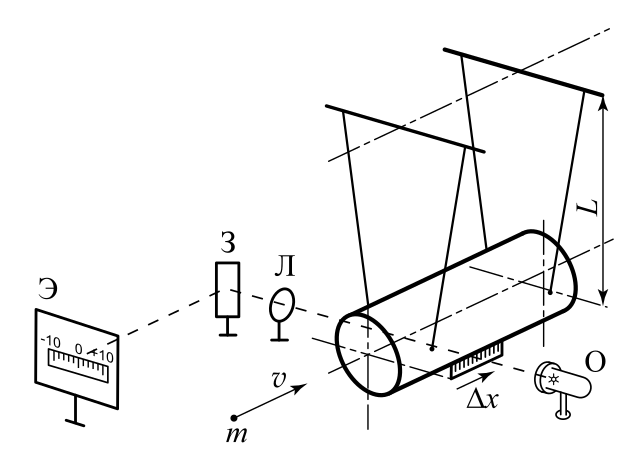
\includegraphics[width=0.75\linewidth]{setting-1.png}
                \caption{Схема установки для измерения скорости полёта пули}
                \label{fig:setting-1}
            \end{figure}

        \subsection{Метод крутильного баллистического маятника}
            Cхема эксперимента изображена на рисунке \ref{fig:setting-2}. Пуля массой $m$ попадает в мишень, укреплённую на стержне $aa$, который вместе с грузами $M$ и проволокой П образует крутильный маятник. Считая удар неупругим, для определения скорости $u$ полёта пули непосредственно перед ударом воспользуемся законом сохранения момента импульса:

            \begin{equation}
                mur = I\Omega,
                \label{eq:6}
            \end{equation}
            где $\Omega$ "--- угловая скорость маятника, $I$ "--- момент инерции маятника.
            
            \begin{figure}
                \centering
                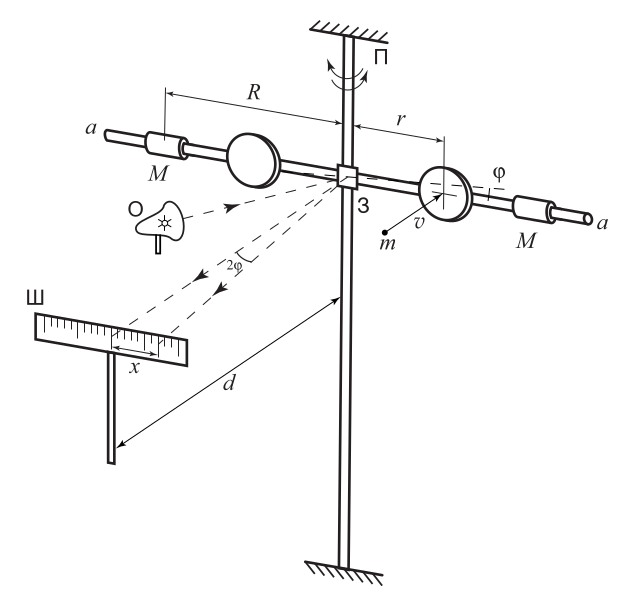
\includegraphics[width=0.75\linewidth]{setting-2.png}
                \caption{Схема установки для измерения скорости пули с крутильным баллистическим маятником}
                \label{fig:setting-2}
            \end{figure}

            Начальная кинетическая энергия переходит в потенциальную, упругую энергию закручивания проволоки, и часть её расходуется на необратимые потери в виде трения о воздух.

            Закон сохранения энергии принимает вид:
            \begin{equation}
                k \frac{\phi^2}{2} = I \frac{\Omega^2}{2},
                \label{eq:7}
            \end{equation}
            где $k$ "--- модуль кручения проволоки П, а $\phi$ "--- максимальный угол поворота маятника.
            Из \ref{eq:6} и \ref{eq:7} получаем
            \begin{equation}
                u = \phi \frac{\sqrt{kI}}{mr}.
                \label{eq:8}
            \end{equation}
            Угол $\phi$ мал и находится по смещению $x$ изображения нити осветителя на шкале:
            \begin{equation}
                \phi \approx  \frac{x}{2d}.
                \label{eq:9}
            \end{equation}

            В формулу \ref{eq:8} входит произведение $kI$, которое можно найти по измерениям периодов колебаний с грузами и без них. В первом случае период равен
            \begin{equation}
                T_1 = 2\pi \sqrt{\frac{I}{k}}
            \end{equation}
            Во втором случае
            \begin{equation}
                T_2 = 2\pi \sqrt{\frac{I-2MR^2}{k}}
            \end{equation}
            Из этих двух равенств следует, что
            \begin{equation}
                \sqrt{kI} = \frac{4\pi MR^2 T_1}{T_1^2 - T_2^2}
                \label{eq:connection}
            \end{equation}

    \section{Ход работы}    
        \subsection{Метод маятника, совершающего поступательное движение}
            Перед проведением эксперимента было проведено знакомство с маятниками, установками и духовым ружьём. Было показано, что при холостом выстреле воздушная струя не оказывает воздействия на маятник.

            Каждая пулька из набора была взвешена и пронумерована, результаты измерений приведены в таблице \ref{table:bullets}. Первые четыре пульки используются во второй части, другие четыре --- в первой.
            
            \begin{table}
                \centering
                \begin{tabular}{|c|c|c|c|c||c|c|c|c|}
                    \hline
                    n & 1 & 2 & 3 & 4 & 5 & 6 & 7 & 8 \\
                    \hline
                    m, г & 0.515 & 0.507 & 0.506 & 0.500 & 0.496 & 0.509 & 0.505 & 0.508 \\
                    \hline
                \end{tabular}
                \caption{Пульки, используемые в работе}
                \label{table:bullets}
            \end{table}

            Далее были измерены параметры установки:
            \begin{itemize}
                \item $M = 2925 \pm 5 \text{ г}$
                \item $L = 217.6 \pm 0.5 \text{ см}$
            \end{itemize}

            Произведём выстрелы по мишеням и обратим внимание на то, что после выстрела положение равновесия маятника смещается, поэтому при расчётах по формуле \ref{eq:speed-1} воспользуемся двумя значениями $\Delta x$: найденными по положениям равновесия до и после выстрела.
            В результате четырёх выстрелов по формуле \ref{eq:speed-1} были получены значения скорости, представленные в таблице. Также была возможность измерить скорость пули с помощью специального прибора.
            Как мы видим, измерения по положениям равновесия после очередного выстрела оказались точнее.
            Найдём среднее значение скорости пули и среднеквадратичную погрешность по формулам
            \begin{align*}
                \mean{u} &= \frac{\sum u_i}{N} \\
                \sigma_\text{случ} &= \sqrt{\frac{\sum{\left( u_i - \mean{u}\right)^2}}{N - 1}} \hspace{1cm} \sigma_{\mean{u}} = \frac{\sigma_u}{\sqrt{N}} \\
                \Delta_\text{сист} &= u \sqrt{\epsilon_m^2 + \epsilon_M^2 + \frac{1}{4} \epsilon_L^2 + \epsilon_{\Delta_x}^2} \\
                \sigma_\text{полн} &= \sqrt{{\sigma_{\mean u}}^2 + {\Delta_u}^2}
            \end{align*}

            \begin{table}
                \centering
                \begin{tabular}{|c|c|c|c|c|}
                    \hline
                    m, г & 0.496 & 0.509 & 0.505 & 0.508 \\
                    \hline
                    $\Delta x = x - x_1, \text{ мм}$ & 9.75 & 9.75 & 9.75 & 7.0 \\
                    \hline
                    $\Delta x = x - x_2, \text{ мм}$ & 10.0 & 10.25 & 10.0 & 7.5 \\
                    \hline
                    $v_1$ & 122.08 & 118.96 & 119.90 & 85.57 \\
                    \hline
                    $v_2$ & 125.21 & 125.06 & 122.98 & 91.69 \\
                    \hline
                    $v_\text{прибор}$ & 124.1 & 126.2 & 113.1 & 94.87 \\
                    \hline
                \end{tabular}
                \caption{Результаты первой части работы}
                \label{table:results-1}
            \end{table}

            Таким образом получаем значение скорости $\mean{u} = 116.2 \pm 24.7 \text{ м} \cdot \text{с}^{-1}$
            
            Среднее значение по прибору $\mean{u} = 114.6 \pm 14.3 \text{ м} \cdot \text{с}^{-1}$

        \subsection{Метод крутильного баллистического маятника}
            Измерим параметры установки:
            \begin{itemize}
                \item $r = 20.5 \pm 0.5 \text{ см}$
                \item $R = 34.0 \pm 0.5 \text{ см}$
                \item $d = 56.0 \pm 0.5 \text{ см}$
                \item массы грузов $M$:
                    \begin{itemize}
                        \item $M_1 = 724.5$ г
                        \item $M_2 = 725.8$ г
                    \end{itemize}
            \end{itemize}

            Чтобы исключить из уравнений модуль кручения проволоки и момент инерции маятника найдём периоды колебаний маятника с грузами и без них по времени 12 колебаний (таблица \ref{table:periods}).

            Проведём серию из четырёх выстрелов и получившиеся отклонения занесём в таблицу \ref{table:results-2}.

            \begin{table}
                \centering
                \begin{tabular}{|c|c|c|}
                    \hline
                    & $T_1$ & $T_2$ \\
                    \hline
                    t, с & 208.1 & 153.5 \\
                    \hline
                    T, с & 17.34 & 12.79 \\
                    \hline
                \end{tabular}
                \caption{Периоды колебаний маятника}
                \label{table:periods}
            \end{table}

            \begin{table}
                \centering
                \begin{tabular}{|c|c|c|c|c|}
                    \hline
                    $m$, г & 0.515 & 0.507 & 0.506 & 0.500 \\
                    \hline
                    $x$, см & 13.7 & 15.0 & 13.0 & 12.0 \\
                    \hline
                    $x_0$, см & -2.25 & -2.25 & -2.5 & -2 \\
                    \hline
                    $u$, м/с & 179.7 & 197.4 & 177.8 & 162.5 \\
                    \hline
                \end{tabular}
                \caption{Результаты второй части работы}
                \label{table:results-2}
            \end{table}

            Найдём теперь скорости пулек с помощью формул \ref{eq:connection}, \ref{eq:9}, \ref{eq:8}:
            \begin{equation*}
                u = \frac{2\pi x MR^2 T_1}{dmr \left(T_1^2 - T_2^2\right)},
            \end{equation*}

            Результаты преведены в таблице \ref{table:results-2}.

            Найдём среднее значение скорости пули и среднеквадратичную погрешность по формулам
            \begin{align*}
                \mean{u} &= \frac{\sum u_i}{N} \\
                \sigma_\text{случ} &= \sqrt{\frac{\sum{\left( u_i - \mean{u}\right)^2}}{N - 1}} \hspace{1cm} \sigma_{\mean{u}} = \frac{\sigma_u}{\sqrt{N}} \\
                \Delta_\text{сист} &= u \sqrt{\epsilon_x^2 + \epsilon_m^2 + \epsilon_M^2 + \epsilon_d^2 + \epsilon_r^2 + 4 \epsilon_R^2 + \epsilon_{T_1}^2 + \frac{\sigma_{T_1}^2 + \sigma_{T_1}^2}{T_1^2 - T_2^2}} \\
                \sigma_\text{полн} &= \sqrt{{\sigma_{\mean u}}^2 + {\Delta_u}^2} \\
            \end{align*}

            В итоге получаем, что $u = 179.4 \pm 9.9 \text{ м} \cdot \text{с}^{-1}$

    \section{Вывод}
        В результате были получены скорости вылета пулек из двух различных ружей двумя различными способами.
        \begin{enumerate}
            \item $u_1 = 116.2 \pm 24.7 \text{ м} \cdot \text{с}^{-1}$
            \item $u_2 = 179.4 \pm 9.9 \text{ м} \cdot \text{с}^{-1}$
        \end{enumerate}

        Разброс измеренных скоростей оказался больше посчитанных погрешностей. Это говорит о том, что скорости вылета пуль заметно меняются от выстрела к выстрелу.

\end{document}